\onecolumn\twocolumn
\section{Evaluation}
\label{sec:eval}

% These top level graphs are based on raw data and pick some select points.
% If you want to see the full tput-latency graphs, uncomment the section of graphs at the bottom

%%%%%%%%%%%%%%%%%%%%%%%%%%%%%%%%%%%%%%%%
%%%%%%%%%%%% Uniform fanout %%%%%%%%%%%%
%%%%%%%%%%%%%%%%%%%%%%%%%%%%%%%%%%%%%%%%
% Single shard p99 + p50
\begin{figure*}[!htb]
\centering
\subfloat[1 shard p99]{
  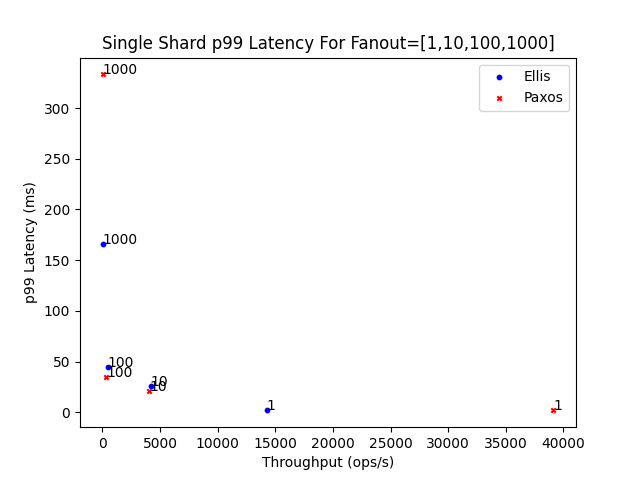
\includegraphics[scale=.2]{figs/1shardp99.png}
  \label{fig:1shardp99}
}
\subfloat[1 shard p50]{
  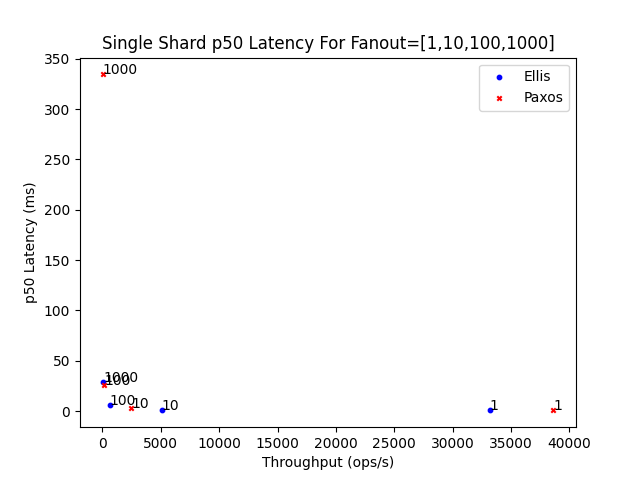
\includegraphics[scale=.2]{figs/1shardp50.png}
  \label{fig:1shardp50}
}
\hspace{0mm}
% 3 shards p99 + p50
\centering
\subfloat[3 shard p99]{
  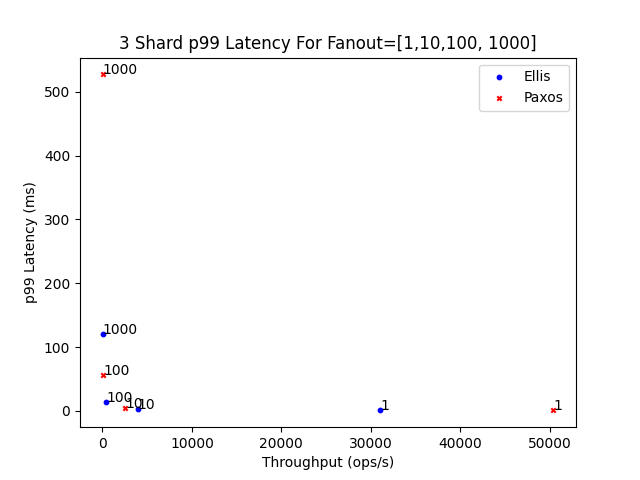
\includegraphics[scale=.2]{figs/3shardp99.png}
  \label{fig:3shardp99}
}
\subfloat[3 shard p50]{
  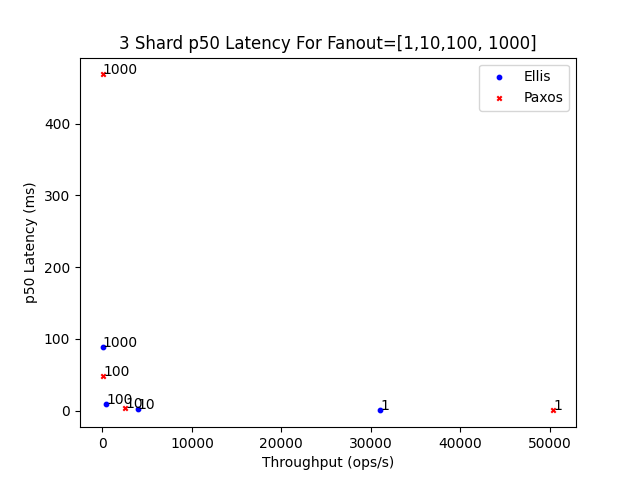
\includegraphics[scale=.2]{figs/3shardp50.png}
  \label{fig:3shardp50}
}
\hspace{0mm}
% 9 shards p99 + p50
\centering
\subfloat[9 shard p99]{
  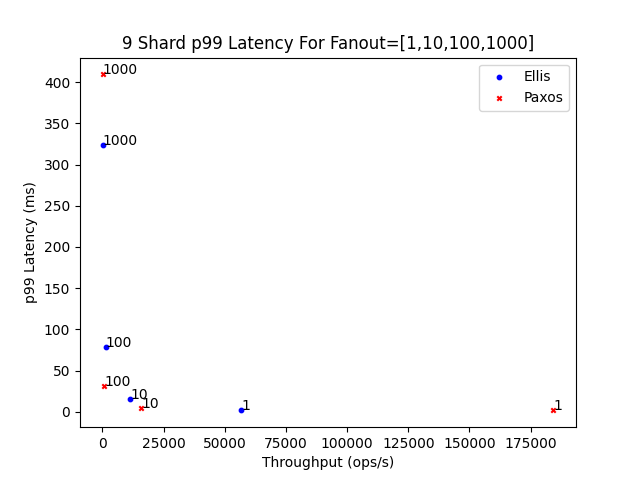
\includegraphics[scale=.2]{figs/9shardp99.png}
  \label{fig:9shardp99}
}
\subfloat[9 shard p50]{
  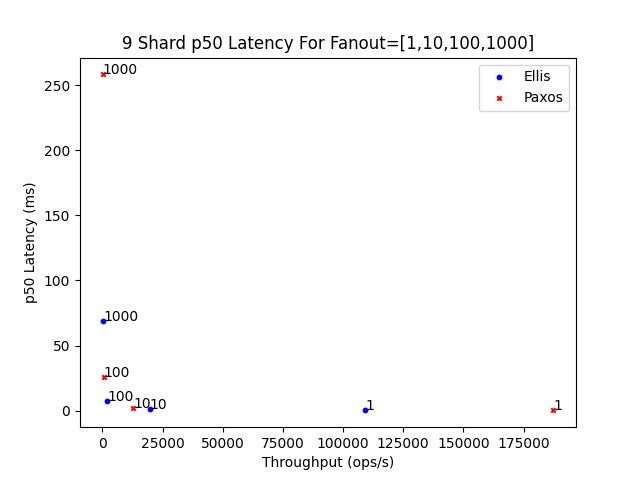
\includegraphics[scale=.2]{figs/9shardp50.png}
  \label{fig:9shardp50}
}
\caption{p99 and p50 for various shard settings.}
\end{figure*}

%%%%%%%%%%%%%%%%%%%%%%%%%%%%%%%%%%%%%%%%
%%%%%%%%%%%% 3 shard skew %%%%%%%%%%%%%%
%%%%%%%%%%%%%%%%%%%%%%%%%%%%%%%%%%%%%%%%
\begin{figure*}[!htb]
\centering
\subfloat[skew\xspace0.5]{
  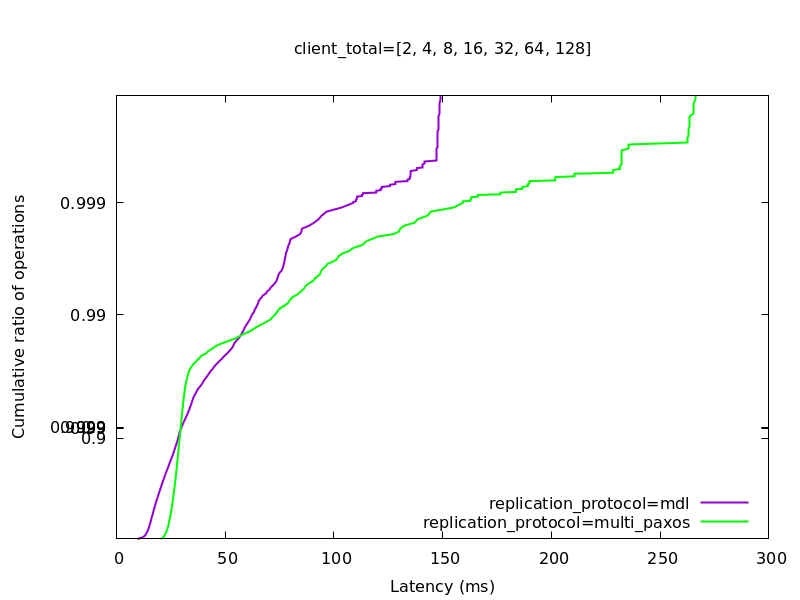
\includegraphics[scale=.1]{figs/3shards_fanout100_skew0.5_16client_CDF.png}
}
\subfloat[skew\xspace0.7]{
  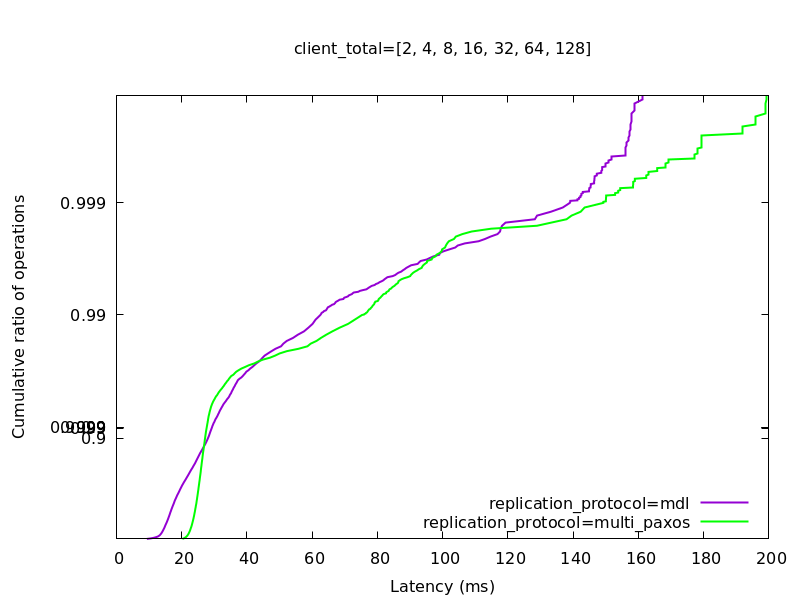
\includegraphics[scale=.1]{figs/3shards_fanout100_skew0.7_16client_CDF.png}
}
\subfloat[skew\xspace0.9]{
  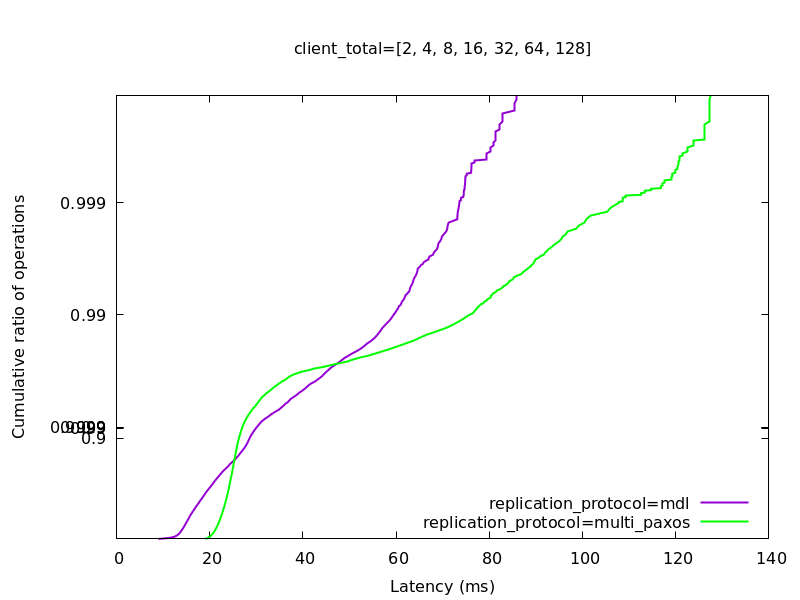
\includegraphics[scale=.1]{figs/3shards_fanout100_skew0.9_16client_CDF.png}
}
\subfloat[skew\xspace1.1]{
  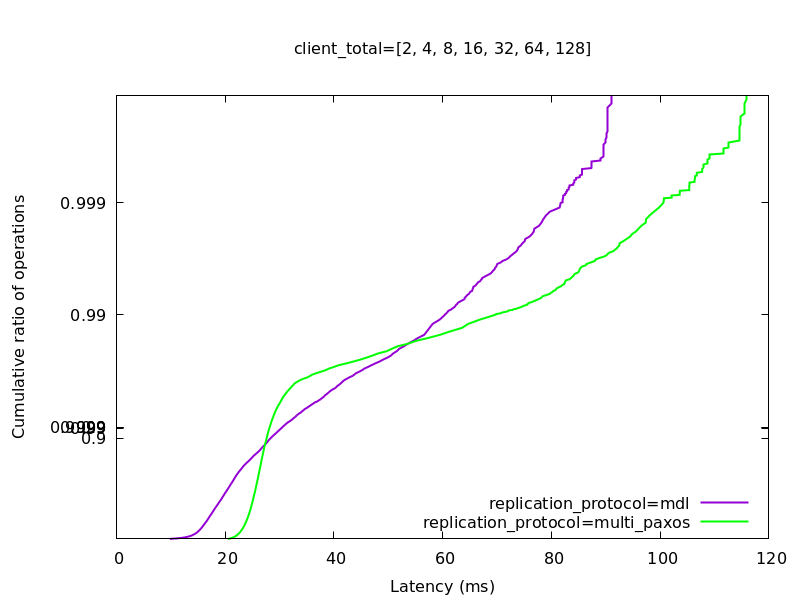
\includegraphics[scale=.1]{figs/3shards_fanout100_skew1.1_16client_CDF.png}
}
\subfloat[skew\xspace1.3]{
  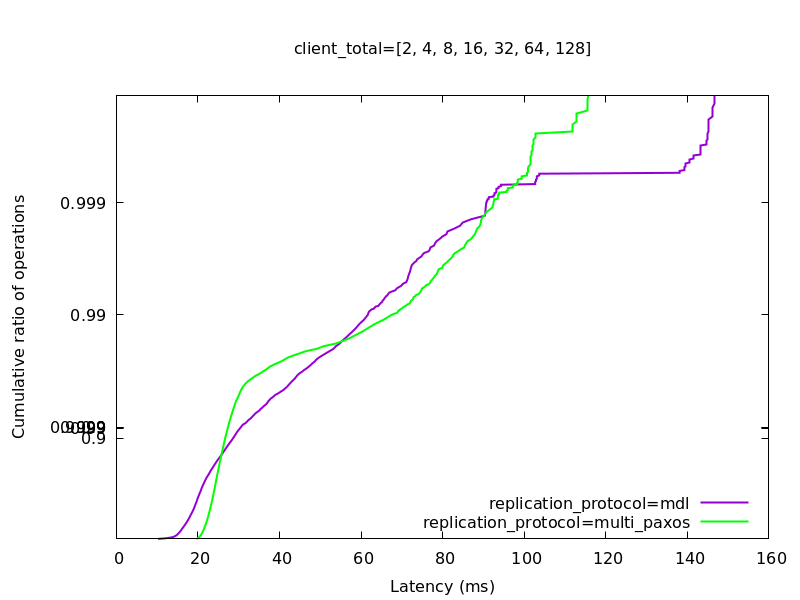
\includegraphics[scale=.1]{figs/3shards_fanout100_skew1.3_16client_CDF.png}
}
\caption{3 shard skew.}
\end{figure*}


%%%%%%%%%%%%%%%%%%%%%%%%%%%%%%%%%%%%%%%%
%%%%%%%%%%%% 9 shard skew %%%%%%%%%%%%%%
%%%%%%%%%%%%%%%%%%%%%%%%%%%%%%%%%%%%%%%%
\begin{figure*}[!htb]
\centering
\subfloat[skew\xspace0.5]{
  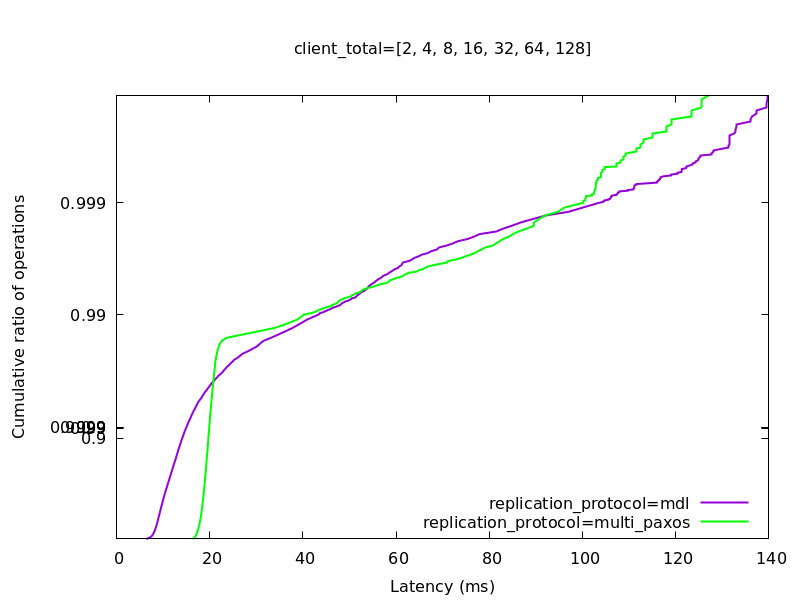
\includegraphics[scale=.1]{figs/9shards_fanout100_skew0.5_16client_CDF.png}
}
\subfloat[skew\xspace0.7]{
  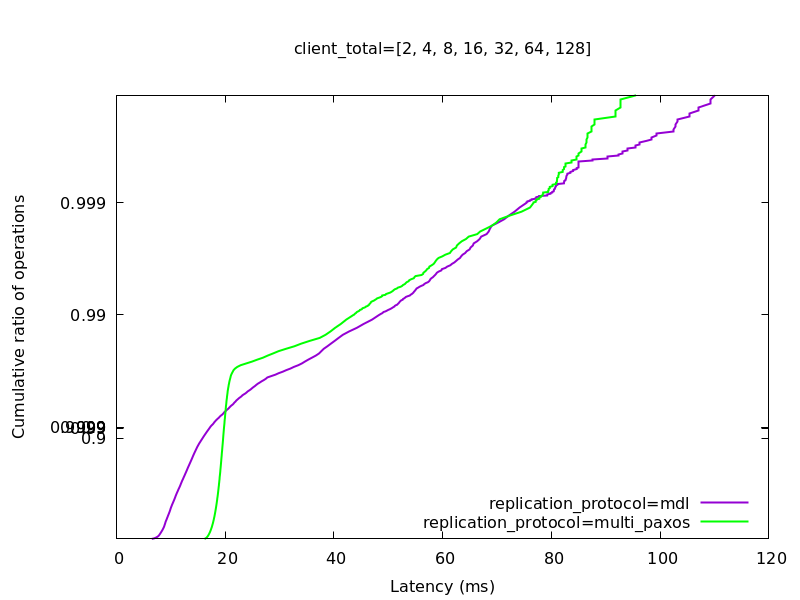
\includegraphics[scale=.1]{figs/9shards_fanout100_skew0.7_16client_CDF.png}
}
\subfloat[skew\xspace0.9]{
  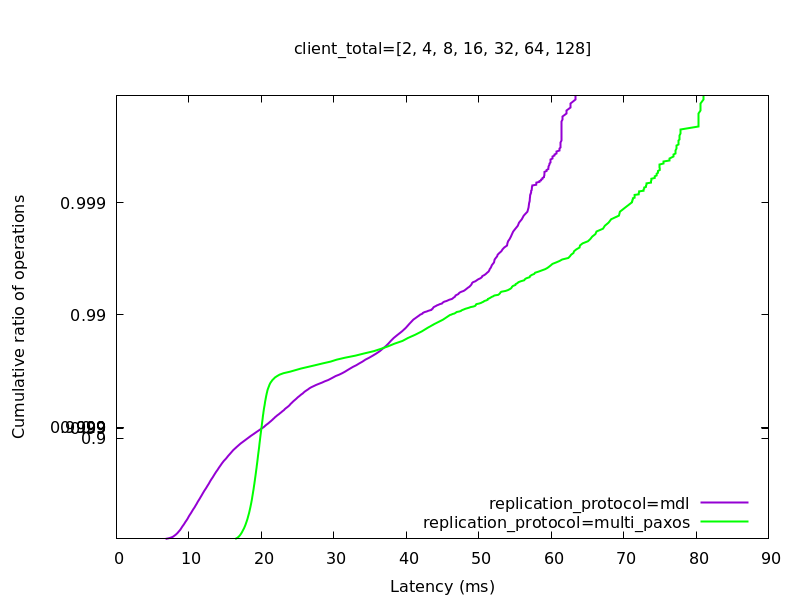
\includegraphics[scale=.1]{figs/9shards_fanout100_skew0.9_16client_CDF.png}
}
\subfloat[skew\xspace1.1]{
  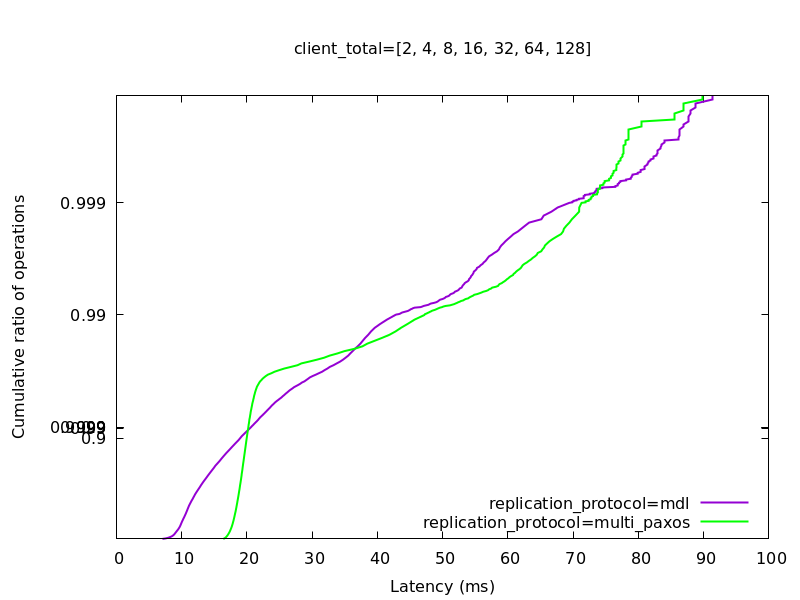
\includegraphics[scale=.1]{figs/9shards_fanout100_skew1.1_16client_CDF.png}
}
\subfloat[skew\xspace1.3]{
  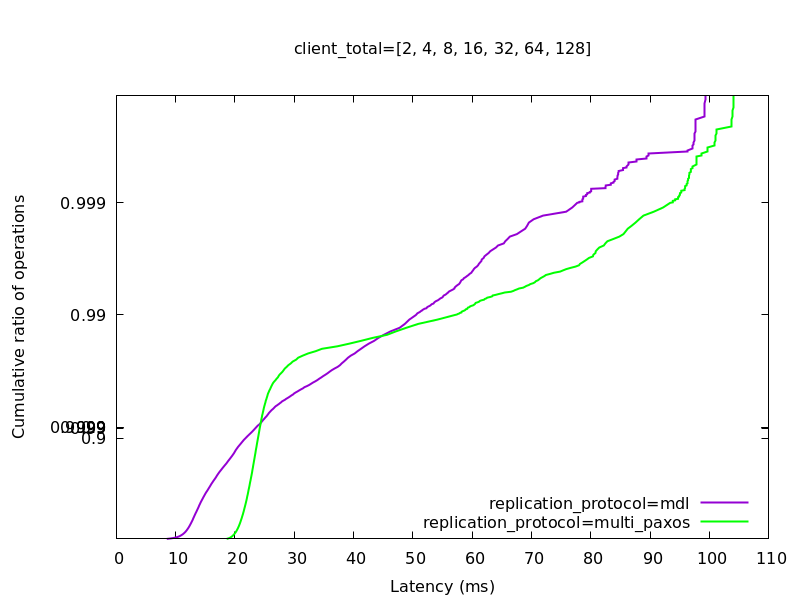
\includegraphics[scale=.1]{figs/9shards_fanout100_skew1.3_16client_CDF.png}
}
\caption{9 shard skew.}
\end{figure*}

%%%%%%%%%%%%%%%%%%%%%%%%%%%%%%%%%%%%%%%%%%%%%%%%%%%%%%%%%%%%%%%%%%%%%%%%%%%%%%%%%%%
%%%%%%%%%%%%%%%%%%%%%%%%%%%%%%%%%%%%%%%%%%%%%%%%%%%%%%%%%%%%%%%%%%%%%%%%%%%%%%%%%%%

%TODO
This section describes how we evaluated \protocol's performance handling requests from multi-dispatch clients compared to \mpaxos's performance handling requests from single-dispatch clients. 
Our focus is on improving end-to-end latency for applications, so we measure application-level request throughput and latency.
We show that our approach achieves improved end-to-end latency for application level-requests, and scales with the number of subrequests issued per application request. 

% Defend choice of metrics -- should this go in another section?
We evaluate both the p99 tail latency as well as p50 median latency. We found that the variability for individual application-level requests was quite high,

\subsection{Experimental Set-up}
All experiments are conducted on Cloudlab's Utah platform ~\ref{}, using m510 machines. 
Our experimental setup consists of a 9-node cluster and 2 client machines. 
Each machine has 1 Intel Xeon-D processor with 8 physical cores running at 2 GHz with hyperthreading enabled, 64 GB of DDR4-2133 RAM, and a 10 Gb/s NIC. 
The roundtrip latency between all machines is around 150 $\mu$s, thus intershard, intrashard, and client-leader latencies are all equal. 
For multi-sharded experiments we evenly distribute replicas across physical machines, placing leaders on different nodes when possible. %TODO

We set the poch length for \system to 1 ms.

\subsection{Client Design}
We evenly distribute client processes across the 2 client machines. Client processes submit application-level requests. Each application-level request submits $n$ system-level subrequests, where $n$ is equal to the fanout parameter for a given experiment. For single-dispatch clients interacting with \mpaxos, only a single system-level subrequest is in-flight at a time, the next subrequest is not issued until the response is received for the preceding subrequest. For multi-dispatch clients interacting with \protocol, all $n$ system-level subrequests are in-flight at the same time, each is submitted in order and does not wait until the response is received for the preceding subrequest.

Each client process is a closed-loop client that submits a single application-level request at a time. The next application-level request is not submitted until all subrequests return. 

In each experiment, we scale the number of clients issueing requests to both systems from 2 to 128 by factors of 2. It's worth noting that since multi-dispatch clients have $n$ requests in-flight at a time, while single-dispatch clients only have 1 request in-flight at a time, \protocol leaders have to deal with $n$ more requests than \mpaxos at any given time for the same number of clients, which is a disadvantage for our system.

%For a fair comparison between MDL and SDL, we keep the number of outstanding requests sent to each system the same. To achieve this, MDL uses a smaller number of clients $K$ with the specified number $N$ of outstanding requests per client, while SDL uses $K*N$ clients each with 1 outstanding request per client.

% \wl{How does keeping the overall number of requests the same mean the load is the same? We discussed this, you can explain this clearly: keep number of outstanding requests the same in both systems, for mdl this uses a smaller number of clients with the specified number of outstanding requests per client, for sdl its N clients with 1 outstanding request per client.}

\subsection{Workload}
We consider uniform and skewed key distributions to explore a more representative range of realistic workloads. For the latter, we generate keys according to a Zipfian distribution with varying skew values $\theta \in \{0.5, 0.7, 0.9, 1.1, 1.3\}$. 

We do not vary the request type at all, all workloads are 100\% writes, since neither our protocol nor basic Paxos implement op-type specific optimizations. 

\subsection{Failures}
We do not consider leader failover in this evaluation. Since failures are rare, and unavoidably degrade performance for most protocols, we only consider the normal mode of operation for \protocol and \mpaxos. Details about the failover specifics in the protocol can be found in ~\ref{sec:design}.

\subsection{Single-Shard}
In this section, we compare the end-to-end application request latency for \system and \mpaxos configured with a single shard. We consider uniform key distribution and vary the fanout parameter.

For each fanout value, we select the number of clients that saturates \system, and plot the p99 and p50 latency for both \system and \mpaxos with that number of clients. Note, this selection for number of clients does not always saturate \mpaxos.

Figures ~\ref{fig:1shardp99} and ~\ref{fig:1shardp50} show the throughput latency curves for ranging fanout values of application-level requests. Since our implementation uses an epoch value of 1ms, \system is unable to outpeform \mpaxos until around fanout = 10. \system outperforms \mpaxos for large fanout values, and 


%discuss relationship between epoch and T, N
%mention that scaling the sdl clients would make us look better.

\subsection{Multi-Shard}
\label{sec:shards}
In this section, we show how the MDL e2e application latency scales with the number of shards. 

%Discuss p99 for 3 shards over range of fanouts
%show the latency improves at 9 shards over range of fanouts
%explain why it's better, what's happening, what overhead we've introduced
%mention that p50 is better.

\subsection{Skew}

Our graphs show skew for fanout = 100 with 16 clients. Overall we don't see much of an impact from skew (that's why we graph the CDFs at some saturated client load).
%show p99 for fanout=100, pick clients = saturation point.... over all 5 skew ranges

\begin{comment}
\subsection{MDL with Geo-rep in the Wide Area}
\label{sec:wide}
We show the e2e app. latency for varying inter-shard latency (which we call the wide area **this might be wrong terminology) and inter-replica latency (which we call geo-replication, also might be wrong terminology).

\subsection{Applications on MDL}
\label{sec:apps}

As described in prior sections, we built a tool to automatically transform applications built to interact with SDL backends to interact with MDL backends, maintaining external equivalence. In this section we select 3 representative applications, A1, A2, A3, and show that when transformed with our tool, all 3 see an improvement in e2e latency. We use DeathStar to benchmark the applications.

A1 is an application that ....

A2 is an application that ...

A3 is an application that ...

We expect transformed applications that have a large degree of data parallelism and are read heavy running on MDL backends to see the largest e2e latency improvements over their pre-transformed counterparts running on SDL backends.

Jeff is still looking for these applications at the moment -- it would be good to pick applications that are read heavy and some that are mixed. All should include varying degrees of data parallelism, to show how some improve after the transformation more than others.
\end{comment}


%%%%%%%%%%%%%%%%%%%%%%%%%%%%%%%%%%%%%%%%%%%%%%%%%%%%%%%%%%%%%%%%%%%%%%%%%%%%%%%%%%%
%%%%%%%%%%%%%%%%%%%%%%%%%%%%%%%%%%%%%%%%%%%%%%%%%%%%%%%%%%%%%%%%%%%%%%%%%%%%%%%%%%%
%%%%%%%%%%%%%%%%%%%%%%%%%%%%%%%%%%%%%%%%
%%%%%%%% 1 shard uniform p99 %%%%%%%%%%%
%%%%%%%%%%%%%%%%%%%%%%%%%%%%%%%%%%%%%%%%
\begin{comment}
\begin{figure*}[!htb]
\centering
\subfloat[Fanout\xspace1]{
  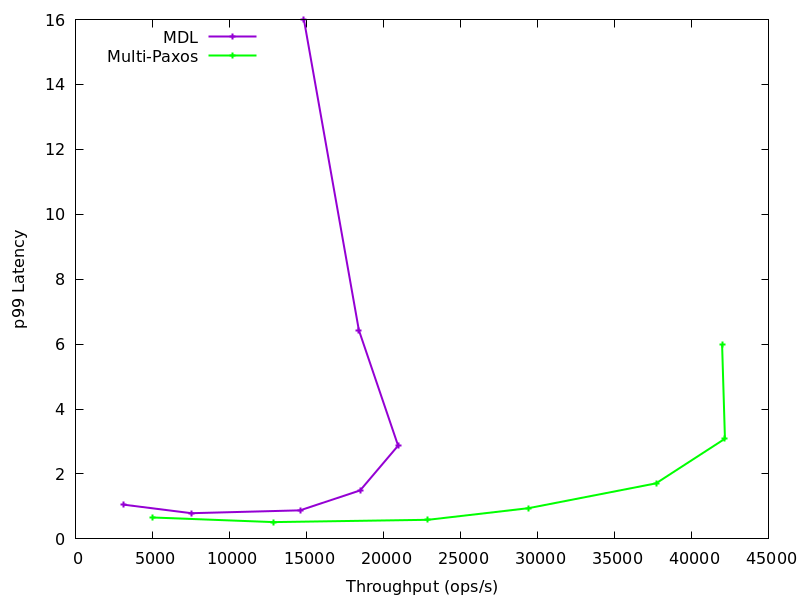
\includegraphics[scale=.15]{figs/1shard_fanout1_p99.png}
}
\subfloat[Fanout\xspace10]{
  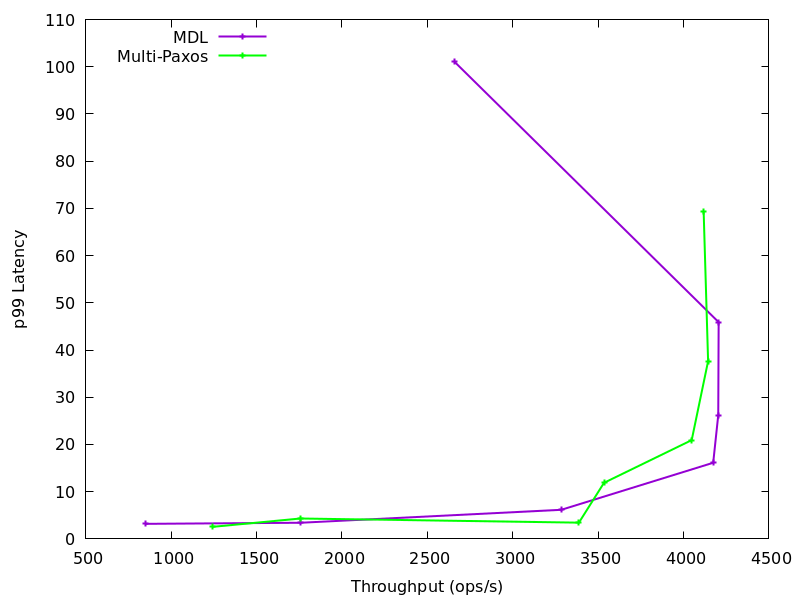
\includegraphics[scale=.15]{figs/1shard_fanout10_p99.png}
}
%\hspace{0mm}
\subfloat[Fanout\xspace100]{
  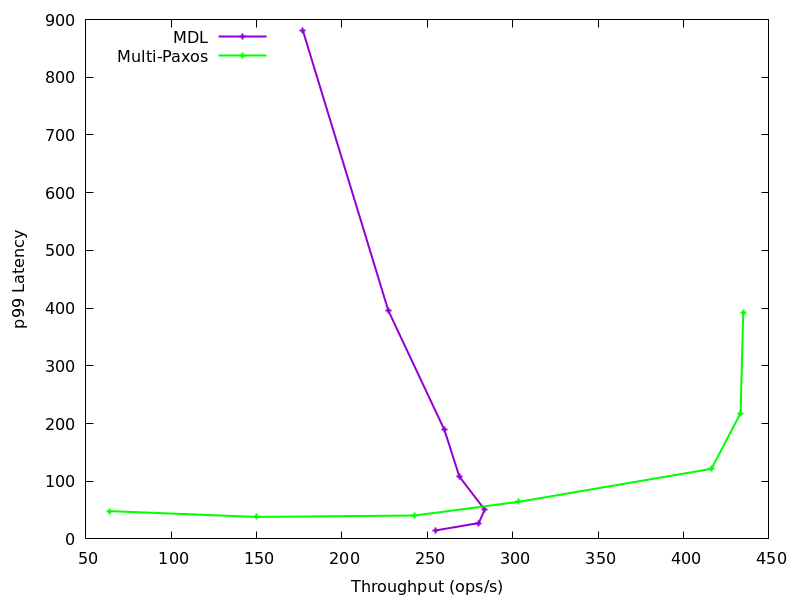
\includegraphics[scale=.15]{figs/1shard_fanout100_p99.png}
}
\subfloat[Fanout\xspace1000]{
  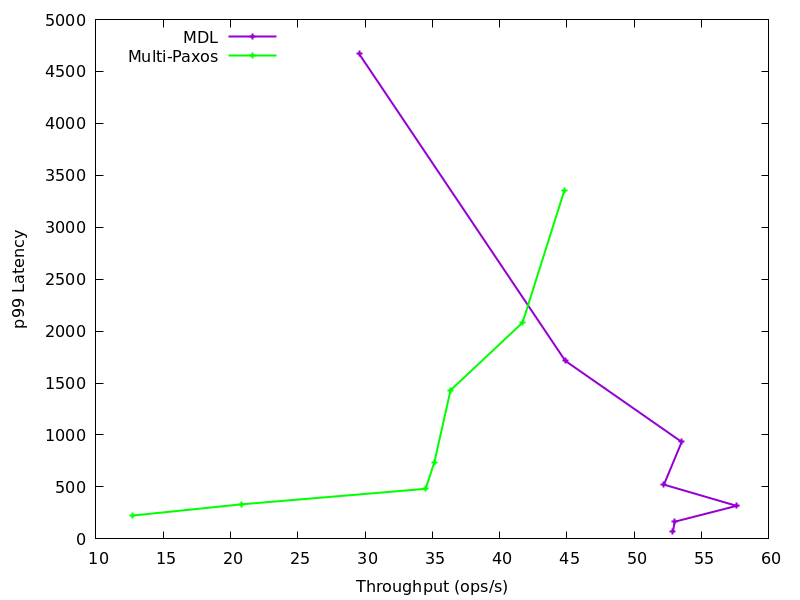
\includegraphics[scale=.15]{figs/1shard_fanout1000_p99.png}
}
\caption{p99 for single shard setting.}
\end{figure*}
%%%%%%%%%%%%%%%%%%%%%%%%%%%%%%%%%%%%%%%%
%%%%%%%% 1 shard uniform p50  %%%%%%%%%%
%%%%%%%%%%%%%%%%%%%%%%%%%%%%%%%%%%%%%%%%
\begin{figure*}[!htb]
\centering
\subfloat[Fanout\xspace1]{
  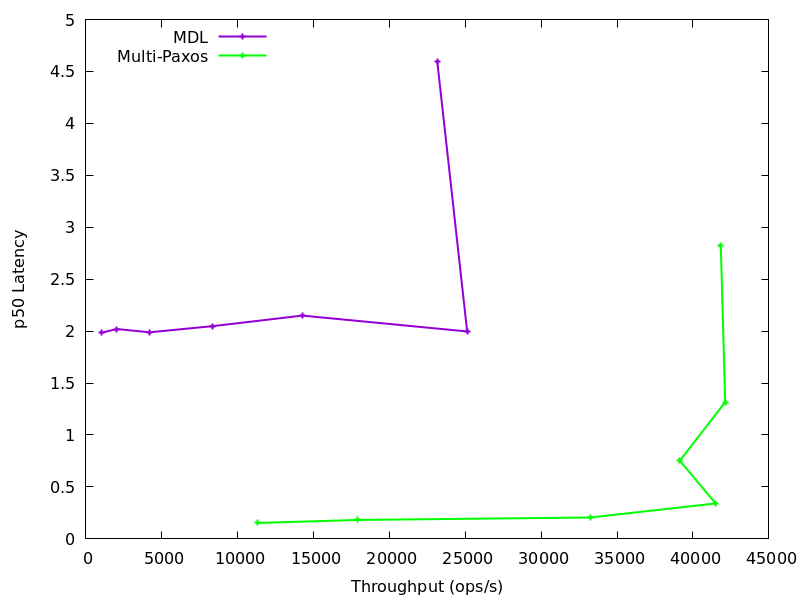
\includegraphics[scale=.15]{figs/1shard_fanout1_p50.png}
}
\subfloat[Fanout\xspace10]{
  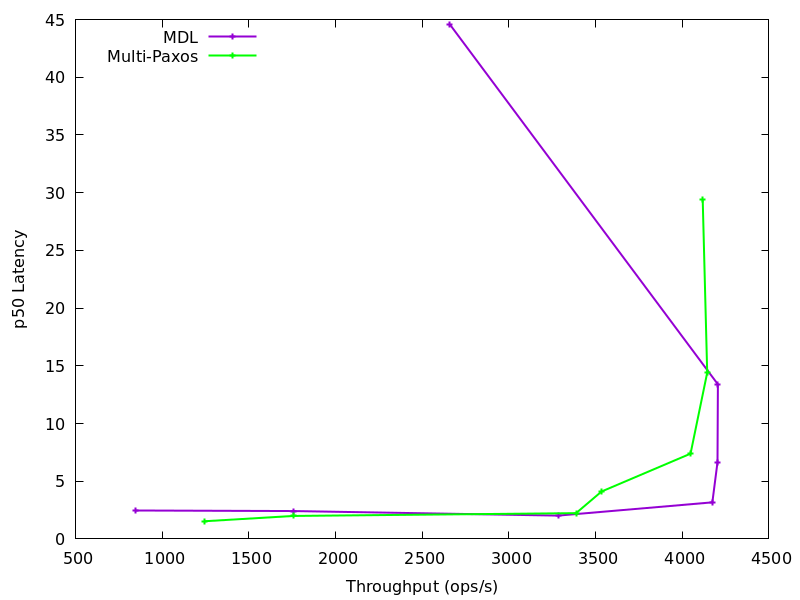
\includegraphics[scale=.15]{figs/1shard_fanout10_p50.png}
}
%\hspace{0mm}
\subfloat[Fanout\xspace100]{
  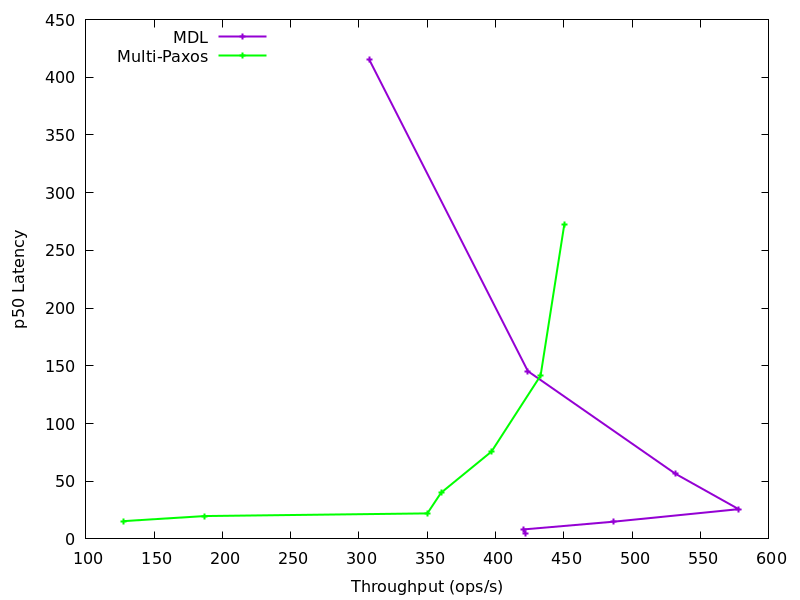
\includegraphics[scale=.15]{figs/1shard_fanout100_p50.png}
}
\subfloat[Fanout\xspace1000]{
  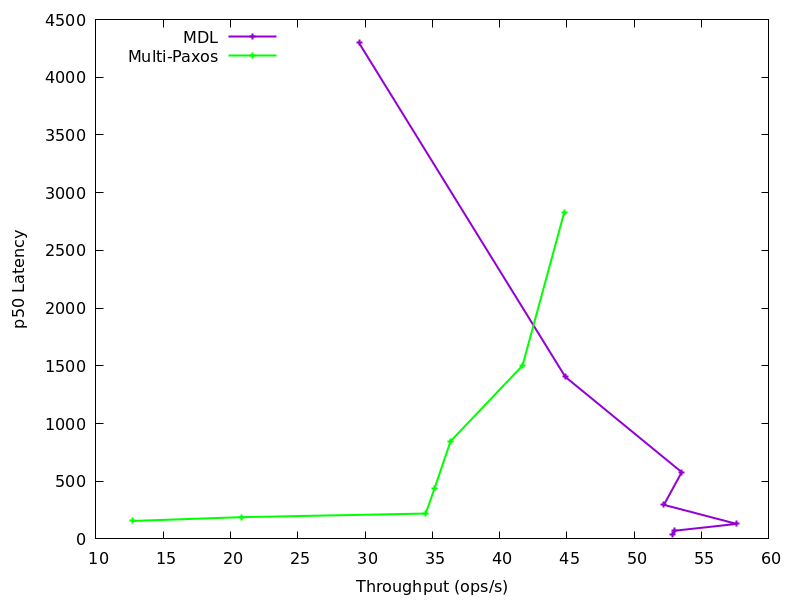
\includegraphics[scale=.15]{figs/1shard_fanout1000_p50.png}
}
\caption{p50 for single shard setting.}
\end{figure*}

%%%%%%%%%%%%%%%%%%%%%%%%%%%%%%%%%%%%%%%%%%%%%%%%%%%%%%%%%%%%%%%%%%%%%%%%%%%%%%%%%%%
%%%%%%%%%%%%%%%%%%%%%%%%%%%%%%%%%%%%%%%%%%%%%%%%%%%%%%%%%%%%%%%%%%%%%%%%%%%%%%%%%%%

%%%%%%%%%%%%%%%%%%%%%%%%%%%%%%%%%%%%%%%%
%%%%%%%% 3 shard uniform p99 %%%%%%%%%%%
%%%%%%%%%%%%%%%%%%%%%%%%%%%%%%%%%%%%%%%%
\begin{figure*}[!htb]
\centering
\subfloat[Fanout\xspace1]{
  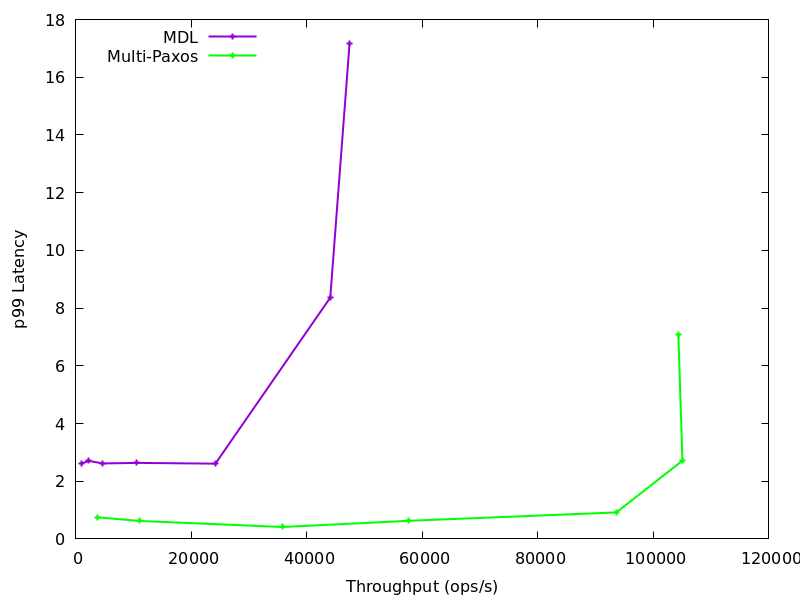
\includegraphics[scale=.15]{figs/3shard_fanout1_p99.png}
}
\subfloat[Fanout\xspace10]{
  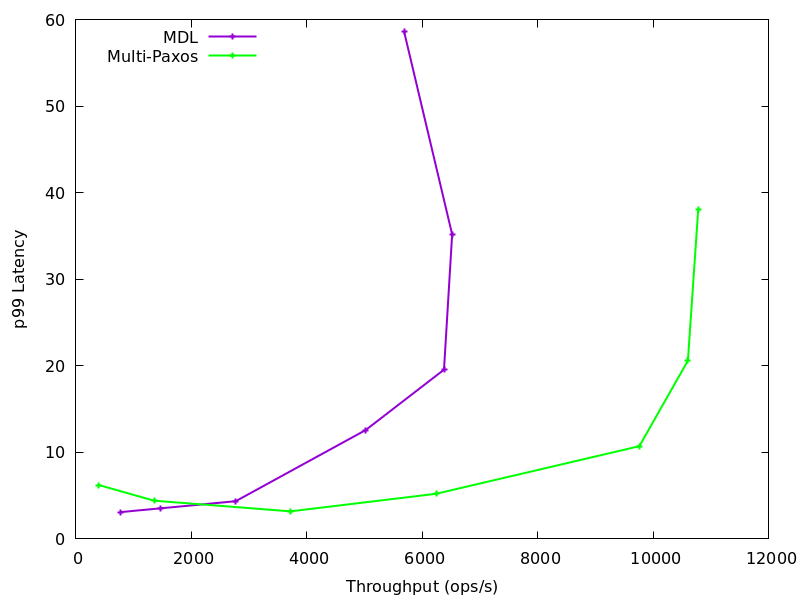
\includegraphics[scale=.15]{figs/3shard_fanout10_p99.png}
}
%\hspace{0mm}
\subfloat[Fanout\xspace100]{
  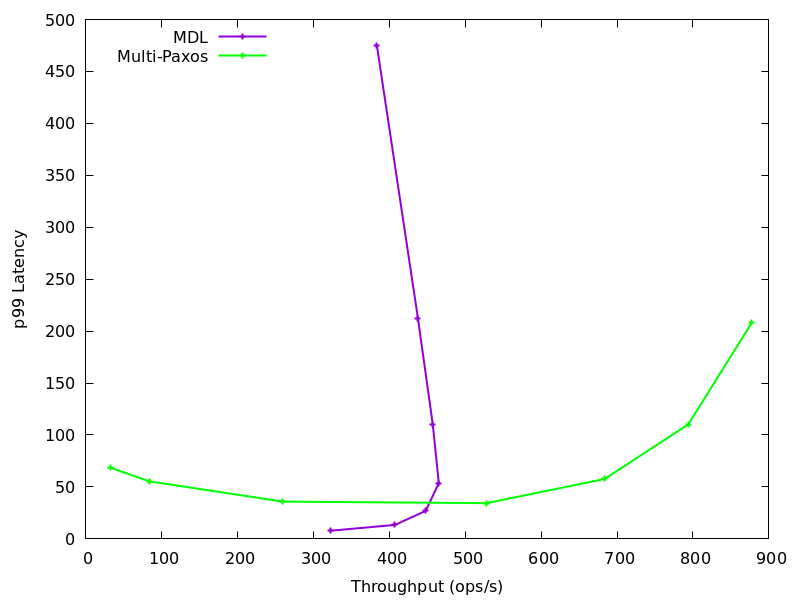
\includegraphics[scale=.15]{figs/3shard_fanout100_p99.png}
}
\subfloat[Fanout\xspace1000]{
  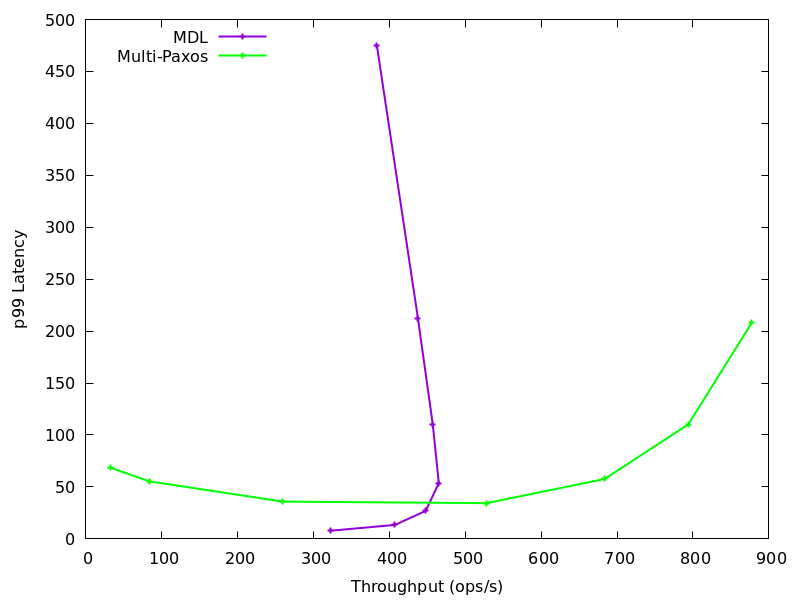
\includegraphics[scale=.15]{figs/3shard_fanout100_p99.png}
}
\caption{p99 for 3 shard setting.}
\end{figure*}

%%%%%%%%%%%%%%%%%%%%%%%%%%%%%%%%%%%%%%%%
%%%%%%%% 3 shard uniform p50  %%%%%%%%%%
%%%%%%%%%%%%%%%%%%%%%%%%%%%%%%%%%%%%%%%%
\begin{figure*}[!htb]
\centering
\subfloat[Fanout\xspace1]{
  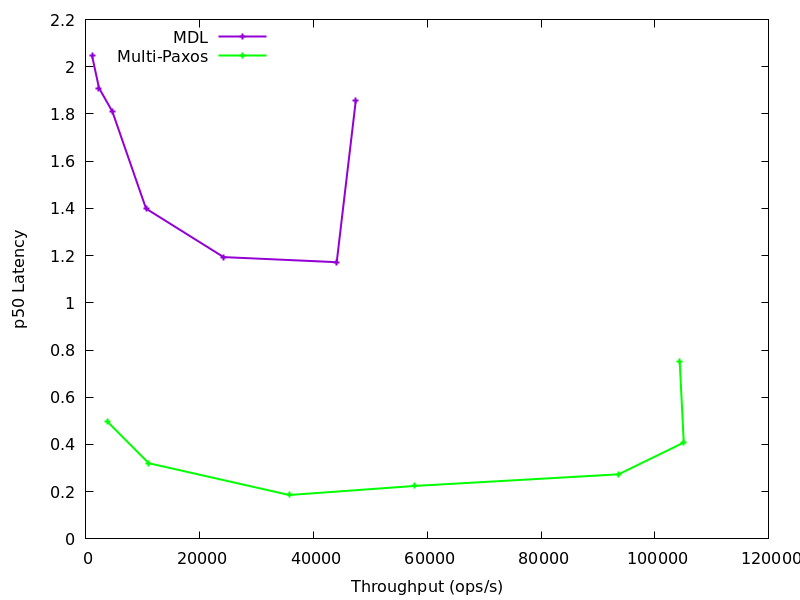
\includegraphics[scale=.15]{figs/3shard_fanout1_p50.png}
}
\subfloat[Fanout\xspace10]{
  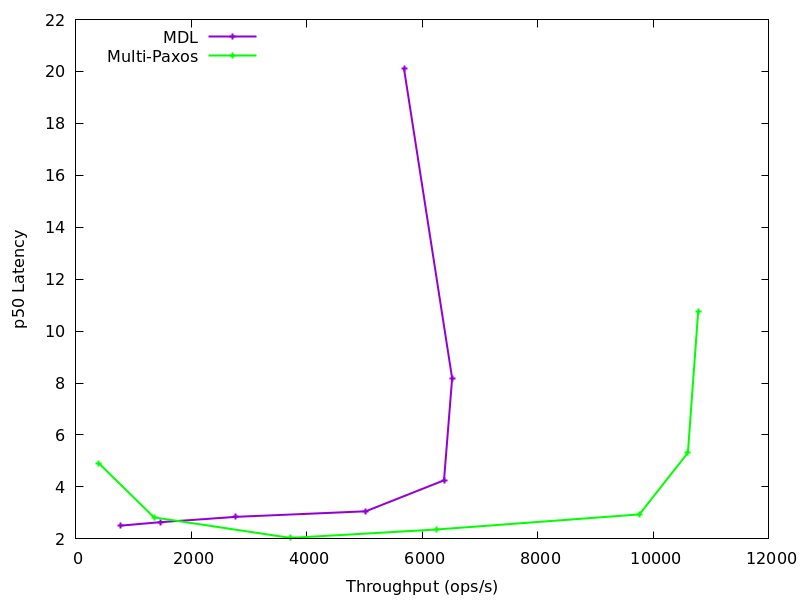
\includegraphics[scale=.15]{figs/3shard_fanout10_p50.png}
}
%\hspace{0mm}
\subfloat[Fanout\xspace100]{
  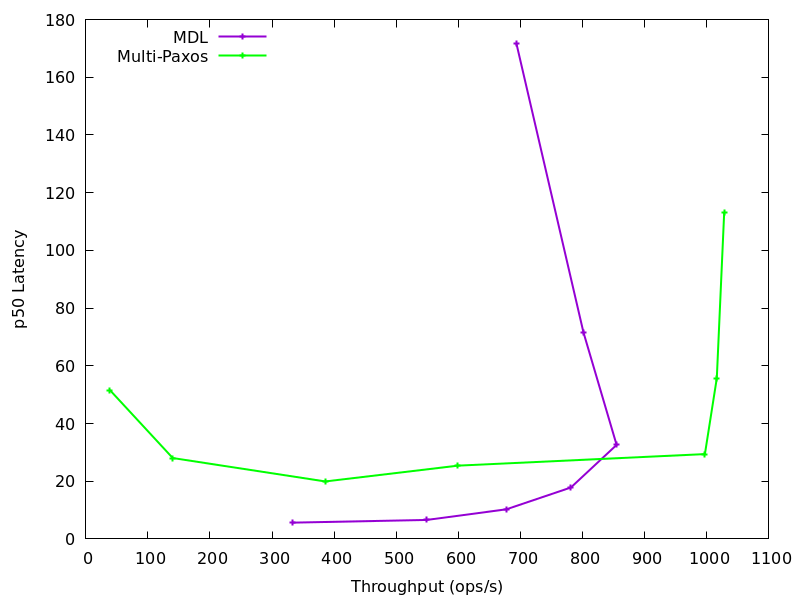
\includegraphics[scale=.15]{figs/3shard_fanout100_p50.png}
}
\subfloat[Fanout\xspace1000]{
  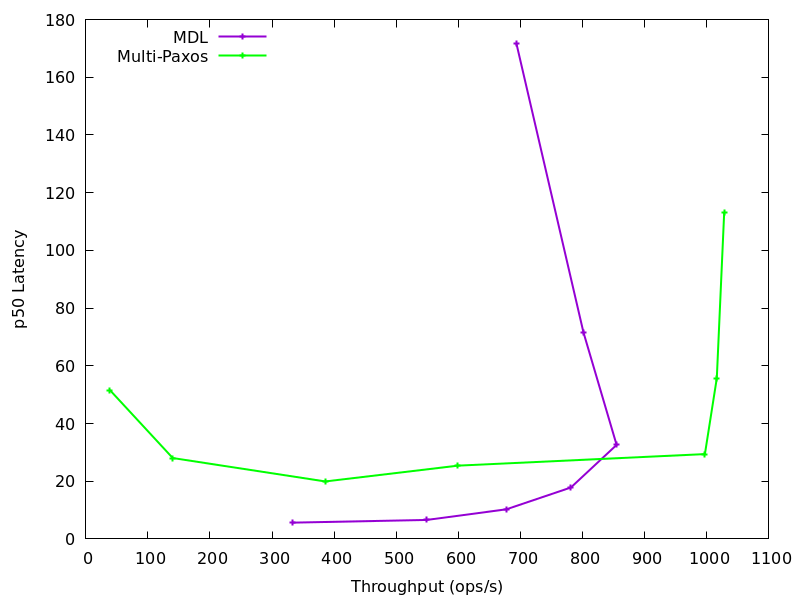
\includegraphics[scale=.15]{figs/3shard_fanout100_p50.png}
}
\caption{p50 for 3 shard setting.}
\end{figure*}


%%%%%%%%%%%%%%%%%%%%%%%%%%%%%%%%%%%%%%%%
%%%%%%%% 9 shard uniform p99 %%%%%%%%%%%
%%%%%%%%%%%%%%%%%%%%%%%%%%%%%%%%%%%%%%%%
\begin{figure*}[!htb]
\centering
\subfloat[Fanout\xspace1]{
  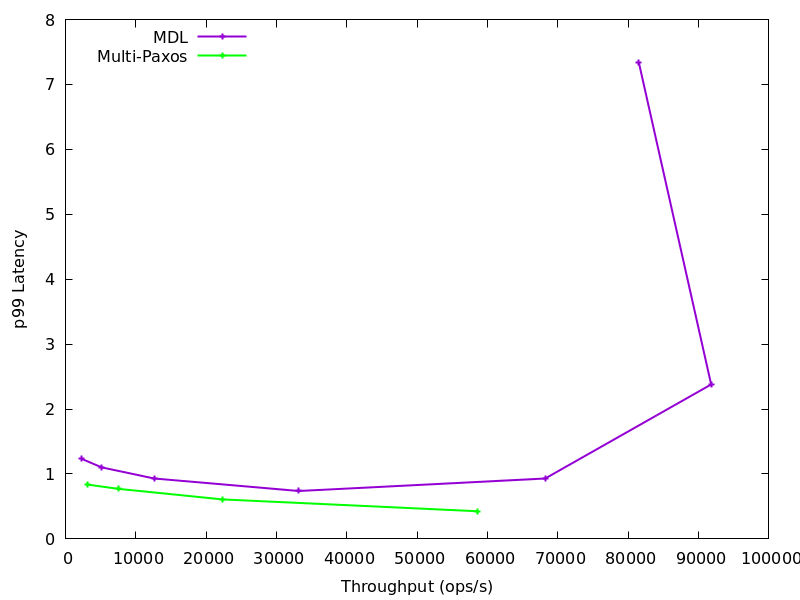
\includegraphics[scale=.15]{figs/9shard_fanout1_p99.png}
}
\subfloat[Fanout\xspace10]{
  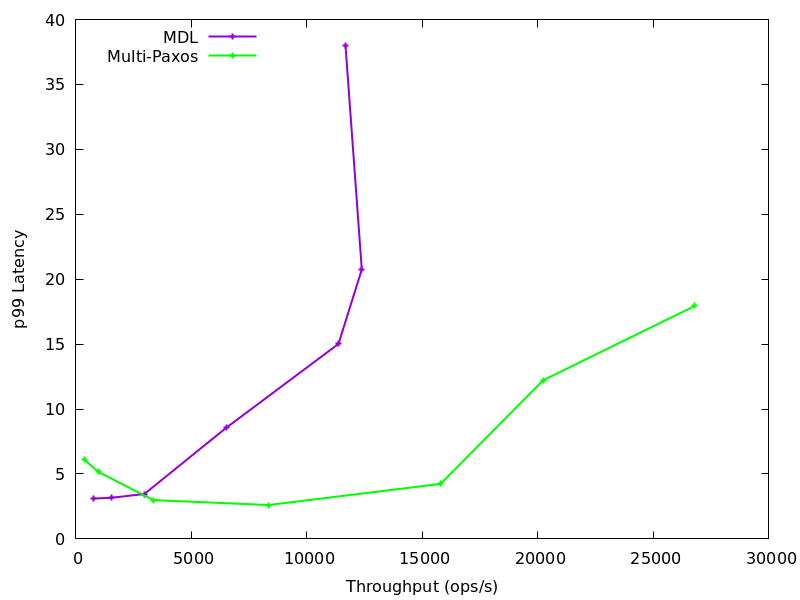
\includegraphics[scale=.15]{figs/9shard_fanout10_p99.png}
}
%\hspace{0mm}
\subfloat[Fanout\xspace100]{
  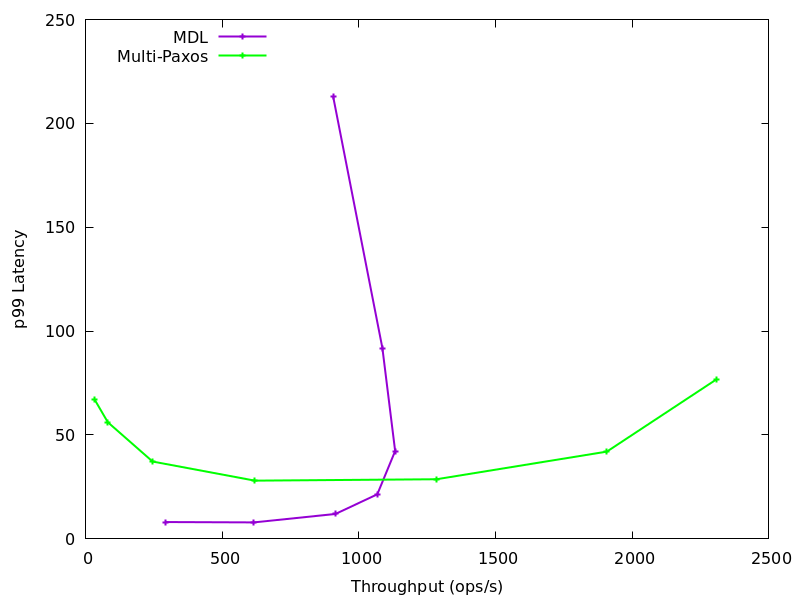
\includegraphics[scale=.15]{figs/9shard_fanout100_p99.png}
}
\subfloat[Fanout\xspace1000]{
  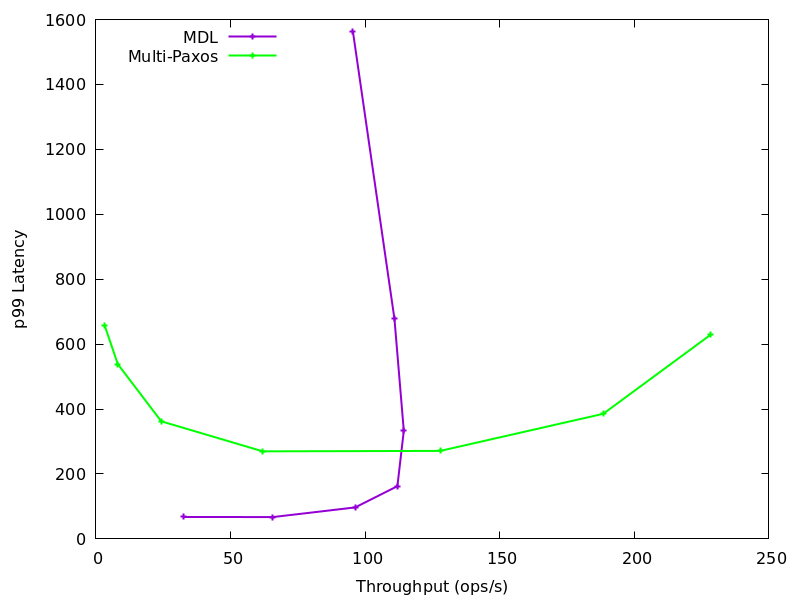
\includegraphics[scale=.15]{figs/9shard_fanout1000_p99.png}
}
\caption{p99 for 9 shard setting.}
\end{figure*}

%%%%%%%%%%%%%%%%%%%%%%%%%%%%%%%%%%%%%%%%
%%%%%%%% 9 shard uniform p50  %%%%%%%%%%
%%%%%%%%%%%%%%%%%%%%%%%%%%%%%%%%%%%%%%%%
\begin{figure*}[!htb]
\centering
\subfloat[Fanout\xspace1]{
  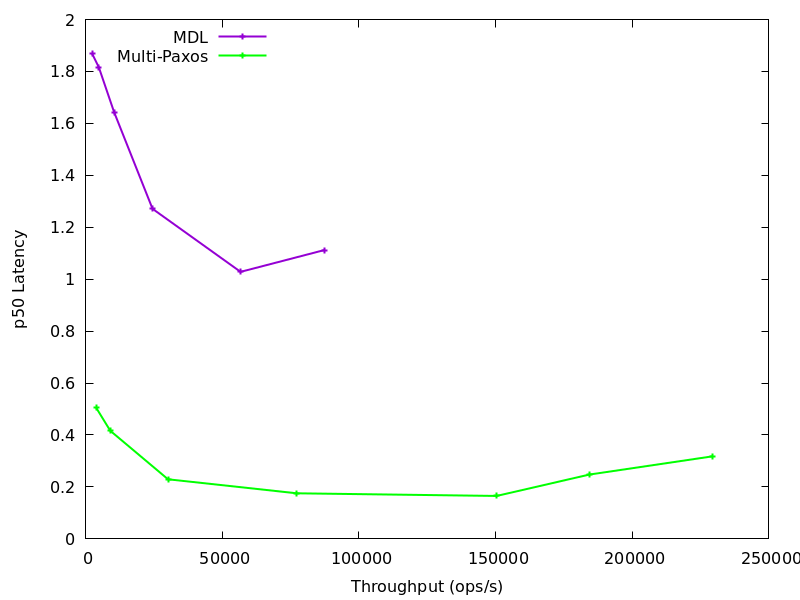
\includegraphics[scale=.15]{figs/9shard_fanout1_p50.png}
}
\subfloat[Fanout\xspace10]{
  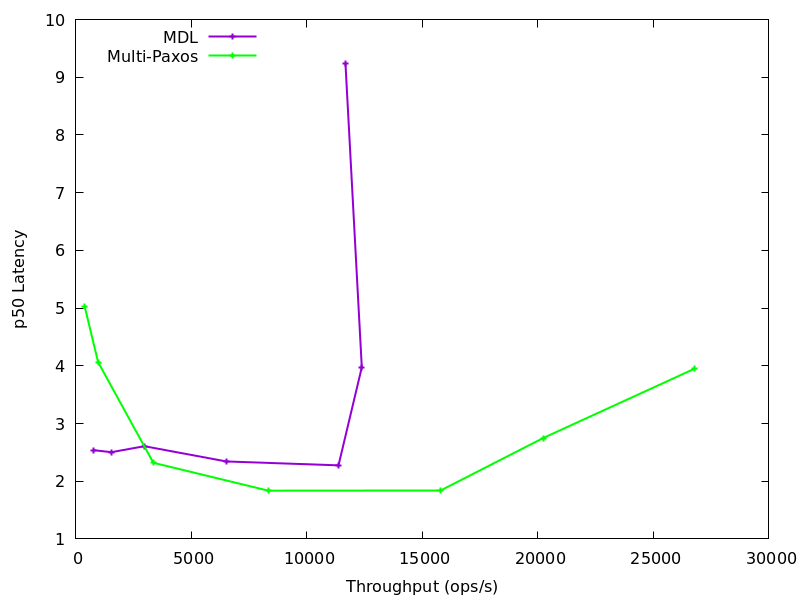
\includegraphics[scale=.15]{figs/9shard_fanout10_p50.png}
}
%\hspace{0mm}
\subfloat[Fanout\xspace100]{
  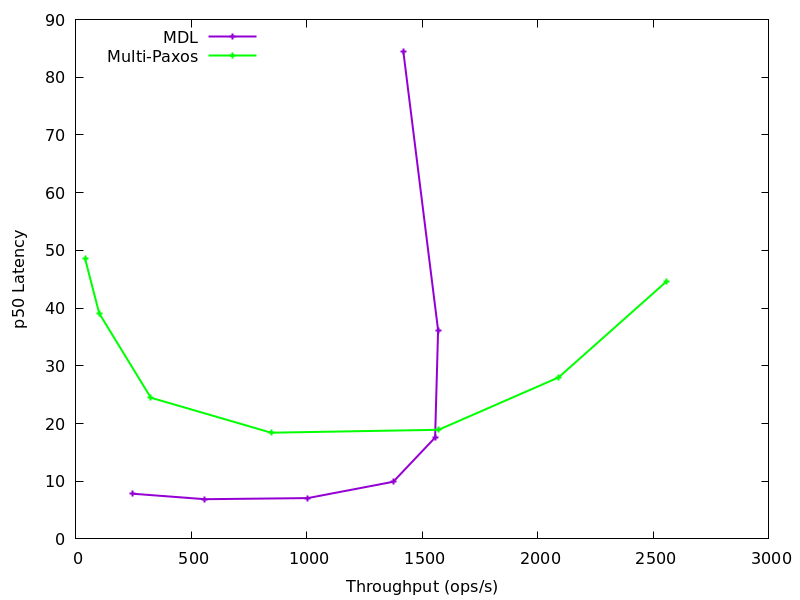
\includegraphics[scale=.15]{figs/9shard_fanout100_p50.png}
}
\subfloat[Fanout\xspace1000]{
  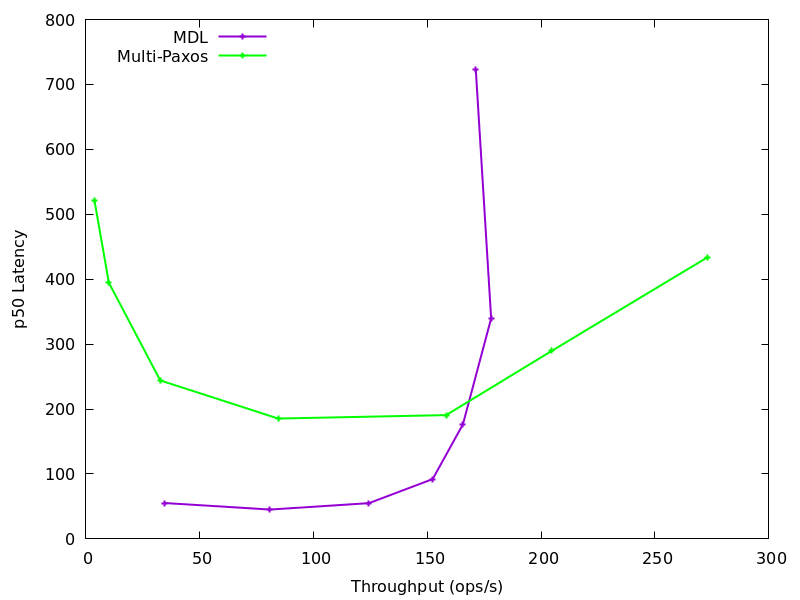
\includegraphics[scale=.15]{figs/9shard_fanout1000_p50.png}
}
\caption{p50 for 9 shard setting.}
\end{figure*}
\end{comment}
%%%%%%%%%%%%%%%%%%%%%%%%%%%%%%%%%%%%%%%%%%%%%%%%%%%%%%%%%%%%%%%%%%%%%%%%%%%%%%%%%%%
%%%%%%%%%%%%%%%%%%%%%%%%%%%%%%%%%%%%%%%%%%%%%%%%%%%%%%%%%%%%%%%%%%%%%%%%%%%%%%%%%%%


